\documentclass[paper=a4,oneside,fontsize=12pt, parskip=full]{scrartcl}
\usepackage{color,soul}
\usepackage[left=1.5cm,right=2.5cm,top=2cm,bottom=1.5cm]{geometry}
\usepackage{tikz-page}
\usepackage{framed}
\usepackage{bm}
\usepackage{tikz}
\usepackage{listings}
\usepackage{xcolor}
\usepackage{amsmath}

\definecolor{codegreen}{rgb}{0,0.6,0}
\definecolor{codegray}{rgb}{0.5,0.5,0.5}
\definecolor{codepurple}{rgb}{0.58,0,0.82}
\definecolor{backcolour}{rgb}{0.95,0.95,0.92}

\lstdefinestyle{mystyle}{
    backgroundcolor=\color{backcolour},
    commentstyle=\color{codegreen},
    keywordstyle=\color{magenta},
    numberstyle=\tiny\color{codegray},
    stringstyle=\color{codepurple},
    basicstyle=\ttfamily\footnotesize,
    breakatwhitespace=false,
    breaklines=true,
    captionpos=b,
    keepspaces=true,
    numbers=left,
    numbersep=5pt,
    showspaces=false,
    showstringspaces=false,
    showtabs=false,
    tabsize=2
}
\lstset{style=mystyle}

\begin{document}
    \section{The Integers}\label{sec:the-integers}
    The most common numbers are those used for counting, namely the numbers

    \[1,2,3,4,\dots\]

    which are called the \textbf{positive integers}.
    Even for counting, we need at least one other number, namely,

    \[0(zero)\]

    For instance, we may wish to count the number of right answers you may
    get on a test for this course, out of a possible 100.
    If you get 100, then all your answers were correct.
    If you get 0, then no answer was correct.
    The positive integers and zero can be represented geometrically on a line,
    in a manner similar to a ruler or a measuring stick:

    \begin{center}
        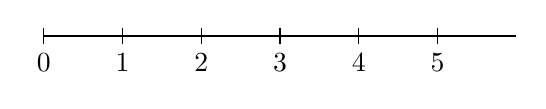
\begin{tikzpicture}
            % Draw the line
            \draw[thick] (0,0) -- (6,0);
            % Draw the ticks and labels
            \foreach \x in {0,1,2,3,4,5} {
                \draw (\x,0.1) -- (\x,-0.1) node[below] {\x};
            }
        \end{tikzpicture}
    \end{center}

    For this we first have to select a unit of distance, say the inch, and then on
    the line we mark off the inches to the right as in the picture.

    For convenience, it is useful to have a name for the positive integers
    together with zero, and we shall call these the \textbf{natural numbers}.
    Thus 0 is a natural number, so is 2, and so is 124,521.
    The natural numbers can be used to measure distances, as with the ruler.

    By definition, the point represented by 0 is called the origin.
    The natural numbers can also be used to measure other things.
    For example, a thermometer is like a ruler which measures temperature.
    However, the thermometer shows us that we encounter other types of numbers besides
    the natural numbers, because there may be temperatures which may go below 0.
    Thus we encounter naturally what we shall call \textbf{negative integers} which
    we call minus 1, minus 2, minus 3, \dots , and which we write as

    \[-1,-2,-3,-4,\dots\]

    We represent the negative integers on a line as being on the other side of 0
    from the positive integers, like this:

    \begin{center}
        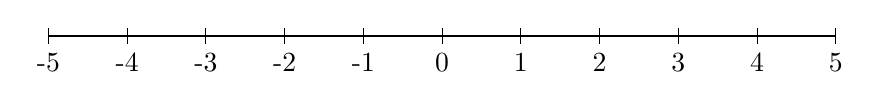
\begin{tikzpicture}
            % Draw the line
            \draw[thick] (-5,0) -- (5,0);
            % Draw the ticks and labels
            \foreach \x in {-5,-4,-3,-2,-1,0,1,2,3,4,5} {
                \draw (\x,0.1) -- (\x,-0.1) node[below] {\x};
            }
        \end{tikzpicture}
    \end{center}

    The positive integers, negative integers, and zero all together are called the integers.
    Thus $-9, 0, 10, -5$ are all integers.

    If we view the line as a thermometer, on which a unit of temperature has
    been selected, say the degree Fahrenheit, then each integer represents a certain temperature.
    The negative integers represent temperatures below zero.

\end{document}